\documentclass{article}

\usepackage[utf8]{inputenc}
\usepackage[czech]{babel}
\usepackage{geometry}
\usepackage{csquotes}
\usepackage{graphicx}
\usepackage{amsthm}
\usepackage{amsmath}
\usepackage{amssymb}

\graphicspath{ { ./ } }

% Define a custom style that removes parentheses
\newtheoremstyle{noparens}
  {3pt}{3pt}                % Space above/below
  {\itshape}                % Body font
  {}                        % Indent amount
  {\bfseries}               % Theorem head font
  { }                       % Punctuation after theorem head
  { }                       % Space after theorem head (changed from \newline)
  {\thmname{#1}\thmnumber{ #2}:\thmnote{ #3}} % Note here without ()

% Define a custom style that removes parentheses
\newtheoremstyle{noparens-mys}
  {3pt}{3pt}                % Space above/below
  {\itshape}                % Body font
  {}                        % Indent amount
  {}               % Theorem head font
  { }                       % Punctuation after theorem head
  { }                       % Space after theorem head (changed from \newline)
  {\textbf{\thmname{#1}\thmnumber{ #2}:}\thmnote{ #3}} % Note here without ()

% Define a custom style that removes parentheses
\newtheoremstyle{noparens-note}
  {3pt}{3pt}                % Space above/below
  {\itshape}                % Body font
  {}                        % Indent amount
  {}               % Theorem head font
  { }                       % Punctuation after theorem head
  { }                       % Space after theorem head (changed from \newline)
  {\thmname{#1}\thmnumber{ #2}:\thmnote{ #3}} % Note here without ()

\theoremstyle{noparens}
\newtheorem*{thm}{Věta}
\newtheorem*{alg}{Algoritmus}
\newtheorem*{anal}{Analýza}
\newtheorem*{ds}{Datová struktura}
\newtheorem*{pozor}{Pozorování}
\newtheorem*{definition}{Definice}
\newtheorem*{heu}{Heuristika}
\newtheorem*{fakt}{Fakt}

\theoremstyle{noparens-mys}
\newtheorem*{anal-mys}{Myšlenky analýzy}
\newtheorem*{alg-mys}{Myšlenky algoritmu}

\theoremstyle{noparens-note}
\newtheorem*{note}{Pozn.}

\newcommand{\OO}{\mathcal{O}}


\title{Příprava na státnicový okruh Grafové algoritmy}
\author{Filip Kastl}
\date{\today}


\begin{document}
\maketitle

\noindent
\textbf{Verze 1}

\noindent
\textbf{Verze 2}: Minimální kostry: Cleanup a pozn., že algoritmy z GA2
netřeba umět.

\noindent
\textbf{Verze 3}: LCA: Oprava časové složitosti makrostuktury.
Karger-Stein: Myslím, že vím jak implementovat vážené hrany.

Tento dokument jsem sepsal zatímco jsem se učil na státnicový okruh Grafové
algoritmy.  Snažím se zde shrnout všechnu látku z magisterských Diskrétních
modelů i bakalářské Obecné informatiky, s kterou jsem se potkal a myslím si, že
spadá do tohoto okruhu.  Je toho opravdu hodně.  Už jsem výběr trochu prořezal
-- odsunul jsem některé věci do druhé sekce.  Pravděpodobně se ale ani všechno
z první sekce nebudu učit.  Každopádně doufám, že tento výčet poslouží mně i
ostatním jako dobrý startovní bod při učení se na státnice.  Hodně štěstí!

\section{O čem se dá mluvit}

\subsection{Pokročilé algoritmy pro nejkratší cesty}

~

\begin{note}
	V tomhle podtématu předpokládáme no negative cycles.
\end{note}

\begin{alg}[Bellman-Ford-Moore]
	$\OO(nm)$, ale umí se vypořádat s negativními hranami
\end{alg}

\begin{thm}
    Dijkstra nikdy znovu neotevře uzavřený vrchol a zavírá vrcholy v pořadí,
    kde neklesá $d(s, v)$.
\end{thm}

\begin{note}
    Dijkstra udělá $\OO(n)\times$ \texttt{Insert}, $\OO(n)\times$
    \texttt{ExtractMin} a $\OO(m)\times$
    \texttt{Decrease}
\end{note}

\begin{center}
\begin{tabular}{ c c c c c }
DS              & \texttt{Insert}           & \texttt{ExtractMin}
                & \texttt{Decrease}         & Dijkstra \\
Pole            & $1$                       & $n$
                & $1$                       & $\OO(n^2)$ \\  
Bin. halda      & $\log n$                  & $\log n$
                & $\log n$                  & $\OO((m + n) \log n)$ \\  
$d$-reg. halda  & $\OO(\log n / \log d)$    & $\OO(d \cdot \log n / \log d)$
                & $\OO(\log n / \log d)$    & $\OO((m + dn) \log n / \log d)$ \\
$m\over n$-reg. halda  & ~ & ~ & ~			& $\OO(m \log n / \log {m\over n})$ \\
Fibbonacci      & $\OO(1)$					& $\OO(\log n)$
				& $\OO(1)$					& $\OO(m + n \log n)$ \\
Délky $\le L$   & $\OO(1)$                  & $\OO(\log L / \log \log L)$
				& $\OO(1)$					& $\OO\left(m + n \cdot {{\log L} \over {\log \log L}}\right)$
\end{tabular}
\end{center}

\begin{note}
    Poslední halda pracuje na celých číslech. Dá se rozšířit i na neceločíselné
    hodnoty, ale pak musím uvažovat $L' := L / \lambda, \forall e: \lambda \le
    l(e) \le L$
\end{note}

\begin{note}
    Na $d := {m\over n}$ jsme přišli tak, že jsme chtěli, aby oba členy ($m
    \cdot \text{zlomek} + n \cdot \text{zlomek}$) byly stejné (to je
    asymptoticky opt.).

	Efektivně se složitost pak volně pohybuje mezi polem a bin. haldou.  Medvěd
    říká, že v praxi je to lepší, než Fibonacciho halda (v té se prý skrývají
    ošklivé konstanty).
\end{note}

\begin{note}
Relaxační algoritmy jako Dijkstra a Bellman-Ford řeší
single-source-shortest-paths.  Medvěd: Vlastně se neví, jak využít toho, že
reálně chceme řešit point-to-point-shortest-path k vylepšení asymptotiky.  Ale
máme heuristiky!
\end{note}

\begin{heu}
    Zastav, když uzavřeš cílový vrchol
\end{heu}
\begin{heu}
    Prohledávej ze zdroje i z cíle najednou (je třeba dokázat)
\end{heu}

\begin{definition}[Potenciál]
    $\varphi: V \rightarrow \mathbb{R}^+_0$
\end{definition}

\begin{definition}[Reduced length]
    $l_\varphi(uv) := l(uv) + \varphi(u) - \varphi(v)$
\end{definition}

\begin{pozor}
    Reduced délka cesty $P$ se zteleskopuje na $l(P) + \varphi(u) -
    \varphi(v)$. Tedy nejkratší cesta je nejkratší i po redukování délek.
\end{pozor}

\begin{definition}[Feasible potenciál]
    $\forall e: l_\varphi(e) \ge 0$
\end{definition}

\begin{thm}
    Pokud no negative cycles, existuje feasible potenciál (pomocí extra vrcholu
    a BFM)
\end{thm}

\begin{note}
    S tímhle potenciálem lze pustit Dijkstru i na grafy s negativními hranami.
\end{note}

\begin{alg}[A*]
    $\psi(v) := \text{dolní odhad na }d(v, t)$.  Zavíráme vždy vrchol s
    nejmenším $h(v) + \psi(v)$ ($h(v)$ je délka dosud nalezené nejkratší cesty
    do $v$).
\end{alg}

\begin{thm}
    A* je ekvivalentní s Dijkstrou s potenciálem $-\psi$
\end{thm}


\subsection{Tranzitivní uzávěr}

\begin{note}
    Zařazuji sem i all-pairs-shortest-paths, protože ty dva problémy úzce
    souvisí.
\end{note}

%\begin{pozor}
%    \enquote{Naivní} tranz. uzávěr: Rychlé mocnění na $n$-tou matice
%    sousednosti $\rightarrow \OO(n^\omega \log n)$.
%\end{pozor}

\begin{pozor}
    Taky bychom mohli prostě $n$-krát iterovat a dostat z Fibonacciho Dijkstry
    $\OO(mn + n^2 \log n)$ APSP (ale FW je lehčí na implementaci) a z BFSka
    $\OO(mn)$ tranz. uzávěr.
\end{pozor}

\begin{alg}[Floyd-Warshal]
    $D_{i,j}^k := \text{$i,j$ vzdálenost pokud povolíme jen }v_i, v_j, v_1,\hdots,v_k$

    $\OO(n^3)$ time, $\OO(n^2)$ space.
\end{alg}

\begin{note}
    FW se dá modifikovat, aby nejen našel vzdálenosti, ale také našel ty cesty.
\end{note}

\begin{note}
    Floyd-Warshal se dá použít pro řešení jiných problémů. Např. nejšiřší
    cesta, nejpravděpodobnější cesta, konstrukce gramatiky pro daný konečný
    automat.

    Trik je v tom nahradit operace. Třeba u nejširší cesty má neexistující walk
    hodnotu $-\infty$, prázdný walk hodnotu $+\infty$, walk o jedné hraně
    prostě šířku té hrany, množina dvou walků maximum šířek těch walků,
    konkatenace dvou walků minimum šířek.

    Pokud bychom chtěli být fancy, uchopili bychom to jako homomorfismy z
    nějaké obecné algebry walků. Tak se to kinda vykládá na GA1. Ale to jde pro
    účely státnic asi moc do hloubky.
\end{note}

\begin{definition}[$(\oplus, \otimes)$-produkt matic.]
    Nechť $\oplus$ je komutativní a asociativní a $\otimes$ je asociativní.

    $$C_{ij} := \bigoplus_k A_{ik} \otimes B_{kj}$$
\end{definition}

\begin{alg}
    $(\lor, \land)$-produkt matic dává $\OO(n^\omega \log n)$ tranz. uzávěr.
\end{alg}

\begin{note}
    $(\min, +)$-produkt matic by dával APSP vzdálenosti, ale protože $\min$
    nemá inverz, nelze použít ty nejchytřejší algoritmy násobení matic, a tak
    zůstáváme na $\OO(n^3 / \log n)$ násobení, s čímž FW nepřekonáme.
\end{note}

\begin{alg-mys}[Seidelův algoritmus]
$\OO(n^\omega \log n)$ full APSP, ale jen pro unweighted
\end{alg-mys}


\subsection{Toky v sítích}

\begin{alg}[Tokové z bakaláře]
~
    \begin{itemize}
        \item Ford-Fulkerson $\OO(nm^2)$ (ale musíme hledat nejkratší
            (neváženou) cestu, také se tomu říká Edmonds-Karpův algoritmus)

        \item Dinic $\OO(n^2m)$

        \item Goldberg $\OO(n^2m)$, asi stačí znát jenom základní princip.
            Hvězdou je tady Dinic.
    \end{itemize}
\end{alg}

\begin{alg}[Dinic s Link/cut stromy $O(nm \cdot \log n)$]
    Prý rychlé i v praxi.
\end{alg}

\begin{anal}[Dinic na jednotkových vahách]
    ~

    \begin{itemize}
        \item $\OO(m^{3 / 2})$
        \item $\Theta(\sqrt{n} \cdot m)$ pro $\min(\deg^{in}(v), \deg^{out}(v)) \le 1$
        \item $\Theta(n^{2/3} \cdot m)$ pro non-multigrafy
    \end{itemize}

    (pro ty $\Theta$ jsme si ukazovali jenom $\OO$ důkaz)
\end{anal}

\begin{alg}[Varianty Dinice pro celočíselné kapacity $\le C$]
    ~

    \begin{itemize}
        \item $\OO(nm + n^2C)$
        \item $\OO(nm \cdot \log C)$
    \end{itemize}
\end{alg}

\begin{note}
    Neprobrané algoritmy:
    \begin{itemize}
        \item 3 indians (varianta Dinice) $\OO(n^3)$
        \item Orlin $\OO(nm)$ (to překonává 3 indy, ty celočíselné algoritmy a
            link-cut trees, ne? leda že oni jsou praktičtější)
        \item V roce 2022 $\OO(m^{1 + \epsilon}), \forall \epsilon \ge 0$
    \end{itemize}
\end{note}


\subsection{Řezy}

\begin{note}
    Pozor na rozdíl mezi libovolným (myslím, že se mu říká \emph{globální})
    řezem a $st$-řezem.

    U globálního řezu uvažujeme neorientovaný
    nevážený graf (Ale Karger-Stein lze upravit pro vážený graf -- složitost
    není závislá na počtu hran, tak prostě použij multihrany, popř. reálná
    čísla jako hran. Myslím, že algoritmus s tímhle v poho bude fungovat.)
\end{note}

\begin{thm}
    Velikost maximálního toku = velikost minimálního $st$ řezu.
\end{thm}

\begin{alg}
    Globální řez pomocí tokového algoritmu najdu tak, že si zafixuji jeden
    vrchol $s$ a pak najdu minimální $st$ řez pro každé $t$.
\end{alg}

\begin{alg}
    Globální separátor (vrcholová souvislost) pomocí tokového algoritmu:
    Rozdělím si každý vrchol na dva.  Ale teď jsem si mohl jako $s$ zafixovat
    jeden z vrcholů separátoru!  Takže zkouším různé volby $s$, dokud nenajdu
    separátor menší než počet $s$, které jsem dosud vyzkoušel.
\end{alg}

\begin{alg}[Contract]
    ~

    \begin{enumerate}
        \item Dokud $n > l$:
        \item ~~~~Vybereneme hranu $e \in E$ rovnoměrně náhodně
        \item ~~~~Zkontrahujeme hranu $e$, smyčky odstraníme, para. hrany
            ponecháme
    \end{enumerate}

    \begin{itemize}
        \item Řez pak najdeme bruteforcem
        \item Celou věc iterujeme -- tomu Wikipedie říká
            \enquote{Kargerův algoritmus}.
    \end{itemize}
\end{alg}

\begin{anal-mys}[Karger]
    ~

    \begin{itemize}
        \item Řez nezničíme s pvd. $c / n^2$, kde $c$ je závislé na $l$. S
            iterováním a $e^{-x} \ge 1 - x$ máme pvd. úspěchu $1 - e^{-cK /
            n^2}$. Pro $K \in \Omega(n^2 \log n)$ stlačíme pvd. neúspěchu pod
            libovolný polynom.
        \item Graf reprezentujeme maticí sousednosti, kde prvky jsou počty
            paralelních hran.
        \item Kontrakce běží v $\OO(n)$, zkontrahování až do $l$ zvládneme v
            $\OO(n^2)$, takže celkem $\OO(n^4 \log n)$ pro inverzně polymiální
            pvd. neúspěchu.
    \end{itemize}
\end{anal-mys}

\begin{alg}[MinCut]
    ~

    \begin{enumerate}
        \item Pokud $n \le 7$, najdeme řez hrubou silou
        \item $l := \lceil n / \sqrt{2} + 1 \rceil$
        \item $C_1 := \text{MinCut}(\text{Contract}(G, l))$
        \item $C_2 := \text{MinCut}(\text{Contract}(G, l))$
        \item Vrátíme menší z $C_1, C_2$
    \end{enumerate}

    \begin{itemize}
        \item Celý Karger-Stein je pak iterování \texttt{MinCut}.
    \end{itemize}
\end{alg}

\begin{anal-mys}[Karger-Stein]
    ~

    \begin{itemize}
        \item Problém se zmenšuje o $\sqrt{2}$, takže $\OO(\log n)$ vrstev rekurze
        \item Nakonec se dobereme k $\OO(n^2 \log n)$ runtimu \texttt{MinCut}
        \item Počítáme pvd. úspěchu na podproblému na $i$-té vrstvě jako
            rekurenci.
        \item Celkově $\OO(n^2 \log^3 n)$ pro inverzně poly. pvd. neúspěchu.
    \end{itemize}
\end{anal-mys}


\subsection{Link/cut stromy}

\begin{ds}[Heavy-light dekompozice (HLD)]
    ~

    \begin{itemize}
        \item Máme váhy buď na hranách nebo na vrcholech
        \item Queries přes cesty (např. minimum)
        \item Bodové (hrana/vrchol) a cestové updaty (např. \enquote{přičti
            $\delta$ všude po cestě})
        \item \emph{Těžká hrana} je ta, na které visí víc jak půlka podstromu.
        \item Základní vlastnosti:
            \begin{enumerate}
                \item Z každého vrcholu dolů vede nejvýše jedna těžká hrana.
                \item Každý vrchol náleží do přesně jedné těžké cesty.
                \item Každá cesta z kořenu do listu obsahuje nejvýše $\log n$
                    lehkých hran.
            \end{enumerate}
        \item Intervalové stromy nad heavy paths $\rightarrow$ path ops v
            $\OO(\log^2 n)$ worst-case (ale tohle Link/Cut stromy překonají).
        \item Pokud nechceme umět updatovat ani strukturu ani váhy,
            můžeme si navíc k intervalovým stromům předpočítat suffixy a
            odpovídat v $\OO(\log n)$.
    \end{itemize}
\end{ds}

\begin{ds}[Link/cut stromy]
    ~

    \begin{itemize}
        \item Dynamická varianta HLD (tedy teď uvažujeme les).
        \item Interface: \texttt{Parent(v), Root(v), Cut(v), Link(u, v),
            Cost(v), PathCost(u, v), SetCost(v), PathUpdate(v, delta),
            Evert(v)} (ten udělá z $v$ kořen)
        \item Jakmile přejdeme na link/cut stromy z HLD, časové složitosti jsou
            amortizované (existuje i worst-case verze, ale Medvěd ji
            neukazoval) -- $\OO(\log n)$
        \item A taky už hranám neříkáme těžké a lehké, ale tlusté a tenké.
        \item A taky už neplatí vlastnost 3.
        \item A taky používáme splay stromy místo intervalových stromů.
        \item Interface operace využívají interní operaci \texttt{Expose(v)} --
            z $v$ udělá první (nejnižší) vrchol tlusté cesty do kořene.
    \end{itemize}
\end{ds}

\begin{anal-mys}[Operace na Link/cut stromech v amort. $O(\log n)$]
    Analýza je založená na analýze splay stromů.  $s(v)$ je tentokrát počet
    descendants včetně těch dosažitelných tenkými hranami.  $r(v) := \log s(v)$
    jako u splay stromů. Naučil bych se asi akorát tolik, aby mi dávalo smysl,
    jak jsou implementované operace.
\end{anal-mys}

\begin{alg}[Dinic s Link/cut stromy $O(nm \cdot \log n)$]
    Prý rychlé i v praxi.
\end{alg}

\subsubsection*{Zdroje}

\begin{verbatim}
Lecture Notes on Data Structures extra chapter "50. Graph data structures"
https://kam.mff.cuni.cz/~mares/video/ls2324/ds2/07-linkcut.mp4
https://kam.mff.cuni.cz/~mares/video/ls2324/ds2/08-linkcut2-semigroup.mp4
https://kam.mff.cuni.cz/~mares/video/ls2526/ds2/06-linkcut.mp4
\end{verbatim}


\subsection{E-T stromy, plně dynamické udržování komponent souvislosti}

\begin{note}
    $(a,b)$-stromy mají $\OO\left({{\log n} \over {\log a}}\right)$
    \texttt{Find} a $\OO\left(b \cdot {{\log n} \over {\log a}}\right)$
    \texttt{Insert} a \texttt{Delete}.
\end{note}

\begin{ds}[E-T stromy]
    ~

    \begin{itemize}
        \item Ukládá Eulerian-Tour sekvence jako listy $(a,b)$-stromů
        \item Nabízí \texttt{Cut}, \texttt{Reroot}, \texttt{Link},
            \texttt{FindRoot}, vše v $\OO(1)$ operacích na $(a,b)$-stromě
        \item Tyhle operace nám přímočaře dávají dynamickou konektivitu na
            lese.
    \end{itemize}
\end{ds}

\begin{note}
    Zatímco Link-Cut stromy nám dávají efektivní operace na cestách, E-T stromy
    nám dávají efektivní operace na podstromech.  Např. některé vrcholy
    původního stromu obarvíme černě.  Info, že vrchol je černý, si udržujeme v
    aktivních externích nodech.  Interní nody si pamatují počet černých vrcholů
    pod sebou.  Pokud chceme vědět, kolik černých vrcholů je v podstromu,
    můžeme ho odříznout a pak se podívat do kořene.  Tohle celé
    je dynamické.  Můžeme měnit barvu vrcholů a můžeme přidávat a ubírat hrany.
\end{note}

\begin{ds}[Dynamická konektivita na grafu (Holme, De Lichtenberg, Thorup)]
    ~

    \begin{itemize}
        \item Jde primárně o zachovávání dvou invariantů
        \item Použijeme-li $a \in \OO(\log n), b \in \OO(a)$, dostaneme DS s
            $\OO\left({{\log n} \over {\log \log n}}\right)$ worst-case query a
            $\OO\left({{\log^2 n}}\right)$ amort. update
    \end{itemize}
\end{ds}

\subsubsection*{Zdroje}

\begin{verbatim}
The Saga of Minimum Spanning Trees (dizertace Martina Mareše): "5.2 Eulerian
Tour trees", "5.3 Dynamic connectivity"
https://kam.mff.cuni.cz/~mares/video/zs2021/ga/2021-01-06.mp4
\end{verbatim}


\subsection{Společní předchůdci ve stromech (LCA)}

\begin{note}
    Lowest Common Ancestor (LCA) úzce souvisí s Range Minimum Query.  RMQ lze
    převést na LCA a to zase lze převést na RMQ$\pm1$ (posloupnost v každém
    bodě roste nebo klesá o $1$). RMQ$\pm1$ pak vyřešíme v $\OO(n)$
    předzpracování a $\OO(1)$ query a tím získáme stejné časy i pro ostatní dva
    problémy.
\end{note}

\begin{pozor}
Pokud se mi nechce předpočítávat, můžu \enquote{paralelně} lézt z obou vrcholů
vzhůru -- $\OO(\min(\text{vzdálenosti těch dvou od LCA}))$
\end{pozor}

\begin{alg}[Převod LCA na RMQ$\pm1$]
    Jednoduchý.
\end{alg}

\begin{alg}[Převod RMQ na LCA]
    Pomocí kartézských stromů.
\end{alg}

\begin{alg}[RMQ$\pm1$]
    ~

    \begin{itemize}
        \item Dekompozice do bloků (velikosti $b := 1/2 \log n$)
        \item Mikrostruktury uvnitř bloků, makrostruktura nad nimi
        \item Mikrostruktura \enquote{bruteforce} předpočítání všech dvojic --
            $\OO(n^2)$ preprocess, $\OO(1)$ query.
        \item Makrostruktura si předpočítá nadbloky obsahující počty bloků
            odpovídající mocninám dvojky (mohou začínat na kterémkoliv indexu)
            -- $\OO(n \log n)$ preprocess, $\OO(1)$ query.
        \item Samozřejmě pak analýza časové složitosti.
    \end{itemize}
\end{alg}

\subsubsection*{Zdroje}

\begin{verbatim}
Krajinou grafových algoritmů str 58, 59
\end{verbatim}


\subsection{Minimální kostry}

~

\begin{alg}[Kostry z bakaláře]
Borůvka, Jarník, Kruskal. Všichni běží v $\OO(m \log n)$ a jsou instancemi
red-blue algoritmu.  Kruskal potřebuje union-find běžící aspoň v $\OO(\log n)$.
\end{alg}

\begin{definition}
    ~

    \begin{itemize}
        \item $T[x, y] := \text{cesta v } T \text{ spojující } x,y$
        \item Hrana $e$ je $T$-light iff $\exists f \in T[e]: w(f) > w(e)$
    \end{itemize}
\end{definition}

\begin{thm}
    $T$ je minimální kostra iff neexistuje $T$-light hrana
\end{thm}

\begin{alg}[Red-blue metaalgoritmus]
Nabarvi nejlehčí hranu elementárního řezu modře nebo
nabarvi nejtěžší hranu cyklu červeně (správnost ez snad krom dokázání, že vše
bude nabarveno).
\end{alg}

\begin{alg}[Kontrahující Borůvka]
  Zahazuje smyčky.  Z paralelních hran vždy zahodí všechny kromě nejtěžší
  (red rule).

  Je třeba rozmyslet, aby kontrakce v každé fázi proběhly v $\OO(m)$. (vypadá ez)
\end{alg}

\begin{anal}[Kontrahující Borůvka $\OO(\min(n^2, m \log n))$]
\end{anal}

\begin{anal}[Kontr. Borůvka s omezenou hustotou]
    Na třídách grafů s konstantou shora omezenou $m / n$ běží v $\OO(n)$
\end{anal}

\begin{fakt}
Minor-closed třídy grafů mají omezené $m / n$. To jsou třeba rovinné grafy.
\end{fakt}

\begin{anal}
Jarník s Fibonacciho haldou $\OO(n \log n + m)$, takže pro třídy grafů s $m / n
    \in \Omega(\log n)$ běží v $\OO(m)$
\end{anal}

\begin{alg-mys}[Fredman-Tarjan]
    Kombinuje chytře Jarníka a kontrahujícího borůvku $\OO(m \cdot \log^* n)$
\end{alg-mys}

\subsubsection*{O následujících algoritmech stačí jen vědět}

\begin{alg-mys}[Verifikace minimality v $O(m)$]
    Používá Borůvka trees, musíme ukázat že stačí lineárně mnoho porovnání vah
    hran a pak ještě algoritmus, který je v lineárním čase najde
\end{alg-mys}

\begin{alg-mys}[Karger-Klein-Tarjan]
    Vychází z verifikace minimality. Expected $\OO(m)$.
\end{alg-mys}

\begin{note}
    ~

    \begin{itemize}
        \item Pettie-Ramachandran je optimální ač nikdo neví, \emph{co} je
            optimální časová složitost. Učili jsme se ho na GA2, ale na
            státnice bych ho úplně vynechal.
        \item Neučili jsme se: $\OO(m)$ pro celočíselné váhy, Chazelle $\OO(m
            \cdot \alpha(m, n))$
    \end{itemize}
\end{note}


\subsection{Testování rovinnosti grafů a kreslení do roviny}

\begin{note}
    ~

    \begin{itemize}
        \item DFS nám spočítá:
        \begin{itemize}
            \item $Enter(v)$ -- kdy DFS vstoupilo
            \item $Ancestor(v)$ -- nejnižší $Enter(u)$ pro zpětné hrany vedoucí z
                $v$ do zpět do $u$
            \item $LowPoint(v)$ -- nejnižší $Ancestor$ podstromu $v$
        \end{itemize}

        \item 2-souvislé \enquote{bloky}.  Mosty v nakreslení zdvojujeme.

        \item \emph{Externí} je zpětná hrana vedoucí do nenakresleného, její
            koncový vrchol, jeho blok a všechny bloky a artikulace nad ním.

        \item \emph{Živý} je koncový vrchol zpětné hrany do zpracovávaného vrcholu
            jeho blok a všechny bloky a artikulace nad ním.

        \item Externí vrcholy nesmíme překlenout. Tomu se bráníme překlápěním
            bloků. Děláme to líně, šetříme tak čas, příznaky v artikulacích.

        \item Pro zrychlení: obcházíme jen živý podgraf.
    \end{itemize}
\end{note}

\begin{alg}[Kreslení do roviny v $\OO(n)$]
    ~

    \begin{enumerate}
        \item Pokud má graf více než $3n - 6$ hran, odmítneme ho rovnou jako
            nerovinný
        \item Prohledáme graf $G$ do hloubky, spočteme \emph{Enter},
            \emph{Ancestor} a \emph{LowPoint} všech vrcholů.
        \item Vytvoříme \emph{BlockList} všech vrcholů přihrádkovým tříděním.
        \item Procházíme vrcholy v pořadí klesajících \emph{Enter}ů, pro každý
            vrchol $v$:
            \begin{enumerate}
                \item Nakreslíme všechny stromové hrany z $v$ jako triviální
                    bloky ($2$-cykly).
                \item Označíme živý podgraf.
                \item Pro každého syna vrcholu $v$ obcházíme živý podgraf
                    náležící k tomuto vrcholu v obou směrech a kreslíme zpětné
                    hrany do $v$.
                \item Zkontrolujeme, zda všechny zpětné hrany vedoucí do $v$
                    byly nakresleny, a pokud ne, prohlásíme graf za nerovinný a
                    skončíme.
            \end{enumerate}
        \item Projdeme hotové nakreslení do hloubky a zorientujeme seznamy
            sousedů.
    \end{enumerate}
\end{alg}

\noindent
\textbf{Pravidlo 1}: V každém živém vrcholu zpracováváme nejdříve zpětné
hrany do $v$, pak podřízené živé interní bloky a konečně podřízené živé
externí bloky.

\noindent
\textbf{Pravidlo 2}: Pokud vstoupíme do dalšího bloku, vybereme si směr, ve kterém
budeme pokračovat, následovně: preferujeme směr k živému internímu vrcholu,
pokud takový neexistuje, pak k živému externímu vrcholu. Pokud se tento
směr liší od směru, ve kterém jsme zatím hranici obcházeli, blok
překlopíme.

\begin{anal-mys}[Když alg. nenakreslí zpětnou hranu, graf není rovinný]
Ukazujeme, že je přítomný $K_5$ nebo $K_{3,3}$ minor

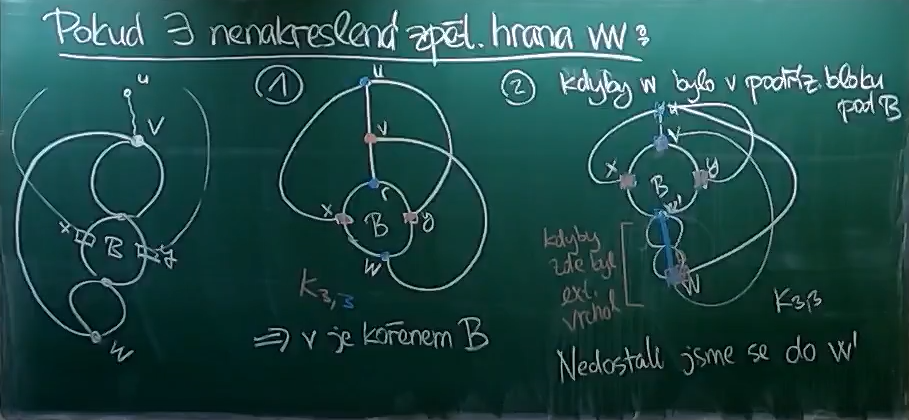
\includegraphics[width=0.9\textwidth]{kresleni-tabule-1.png}

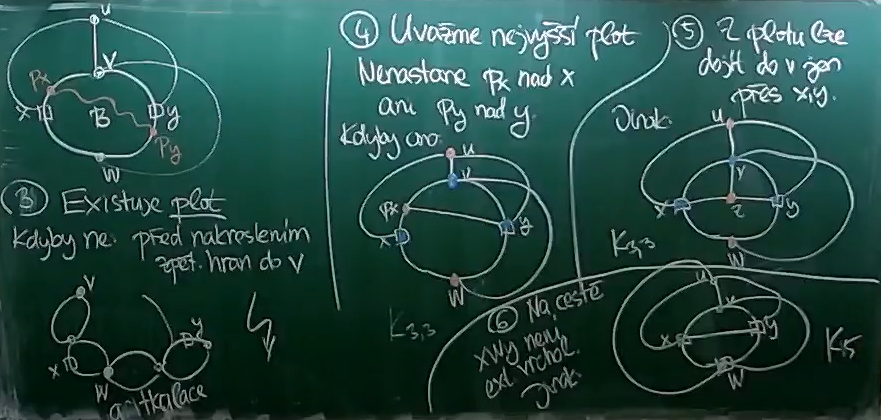
\includegraphics[width=0.9\textwidth]{kresleni-tabule-2.png}
\end{anal-mys}

\subsubsection*{Zdroje}

\begin{verbatim}
Krajinou grafových algoritmů: Kapitola 11
https://kam.mff.cuni.cz/~mares/video/ls2526/ga2/02-rovinne-kresleni.mp4
\end{verbatim}


\subsection{Union-find}

\begin{note}
    Používáme $n$ pro počet vrcholů, na kterých pracujeme a $m$ pro počet operací,
    které provádíme.  Pokud začínáme s izolovanými vrcholy, $n \in \OO(m)$ a
    složitosti se pak zjednoduší na $\OO(\log n)$ nebo $\OO(\alpha(n, n))$ za
    operaci.
\end{note}

\begin{anal}[Union by rank $\OO(\log n)$ na operaci]
    Stromeček ranku $r$ má alespoň $2^r$ vrcholů. (Indukcí, jediný způsob jak
    zvětšit stromeček ranku $r-1$ na $r$ je unionovat k němu další stromeček
    ranku $r-1$)
\end{anal}

\begin{anal-mys}[Path compression $\OO((n + m) \log n)$ (TODO nebo celou
    analýzu?)]
    ~

    \begin{itemize}
        \item Představujeme si, že nejprve provedeme uniony a pak komprese
        \item Indukce přes partition lesu na top a bottom část
        \item Partitionuji na půlky a to mi dá logaritmus
    \end{itemize}
\end{anal-mys}

\begin{definition}[Inverzní Ackermanova funkce]
    ~

    \begin{itemize}
        \item $f^*(n) := \text{kolikrát je třeba aplikovat } f \text{ na }
            n\text{, abych dostal } 1$
        \item $\alpha(m, n) := \text{kolik hvězdiček, abych dostal }
            \log^{**\hdots*}(n) \le {m \over n}$
    \end{itemize}
\end{definition}

\begin{note}
    Toto je jedna z více možných definic $\alpha$.
\end{note}

\begin{anal-mys}[Path compression + union by rank $\OO(\alpha(m, n)m + n)$]
    Používám stejné lemma jako pro analýzu path compression, ale tentokrát
    partitionuji nějak podle ranků
\end{anal-mys}

\subsubsection*{Zdroje}

\begin{verbatim}
https://kam.mff.cuni.cz/~mares/video/ls2122/ds2/09-union-find.mp4
\end{verbatim}


\subsection{Párování}

\begin{note}
    V tomhle podtématu bych se snažil co nejvíc mluvit o tocích.  Kromě nich
    jsem algoritmické teorie párování na magistrovi moc neviděl (vlastně
    žádnou).
\end{note}

\begin{note}
    Uvažujeme maximální párování co do počtu hran v párování. Maximální co do
    inkluze lze získat hladově.
\end{note}

\begin{alg}[Maximální párování v bipartitním grafu pomocí toku]
    Zdůvodnění je látka z bakaláře.  Pomocí $\min(\deg^{in}(v), \deg^{out}(v))
    \le 1$ Dinice v $\OO(\sqrt{n} \cdot m)$.  Vážený případ by se taky řešil
    pomocí toků, ale už ne tak rychle.
\end{alg}

\begin{thm}[Kőnigova]
    V bipartitních grafech velikost největšího párování = velikost nejmenšího
    pokrytí.
\end{thm}

\begin{alg-mys}[Blossom algorithm]
    ~
    
    \begin{itemize}
        \item Mělo by snad stačit vědět, jak zhruba funguje a že existuje.  Učí
            se na bakaláři, ne v GA1, GA2 ani DS2.
        \item Mám maximální párování právě tehdy když v grafu není alternující
            cesta
        \item Při hledání alternujících cest nám nějak překážejí blossoms --
            liché alternující cykly, z kterých vede zpárovaná hrana
        \item Blossoms kontrahujeme a dekontrahujeme
        \item $\OO(e \cdot v^2)$
    \end{itemize}
\end{alg-mys}

\subsubsection*{Zdroje}

\begin{verbatim}
Tomáš Sláma: The Blossom Algorithm
https://www.youtube.com/watch?v=3roPs1Bvg1Q
\end{verbatim}


\newpage
\section{Kdyby toho bylo málo (haha)}

\subsection{Pokročilé algoritmy pro nejkratší cesty}
\begin{itemize}
    \item Tady je variabilita v tom, jak moc se chci učit důkazy všech těch vět
        (každý sám o sobě je vlastně v pohodě) a jak detailně se chci učit tu
        haldu pro délky $\le L$.
\end{itemize}

\subsection{Tranzitivní uzávěr}
\begin{itemize}
    \item Umět detailně popsat walk algebru a její použití
    \item Naučit se Seidelův algoritmus do detailu
\end{itemize}

\subsection{Toky v sítích}
\begin{itemize}
    \item S vylepšením, které jsme neprobírali ale je v průvodci, Goldberga
        dostaneme na $\OO(n^2 \sqrt{m})$
\end{itemize}

\subsection{Řezy}
\begin{itemize}
    \item Nagamochi-Ibaraki -- deterministický $O(mn)$ algoritmus pro nalezení
        globálního minimálního řezu dokonce na váženém grafu. Je popsaný v
        Krajinou grafových algoritmů. Ale na GA1, GA2 ani DS2 se v posledních
        letech neučil.
\end{itemize}

\subsection{Link/cut stromy}
\begin{itemize}
    \item Naučit se amort. analýzu do detailu
\end{itemize}

\subsection{E-T stromy, plně dynamické udržování komponent souvislosti}

\subsection{Společní předchůdci ve stromech (LCA)}
\begin{itemize}
    \item LCA se dá počítat pomocí HLD.  Ale má to horší složitost: $\OO(n)$
        preprocessing a $\OO(\log n)$ query.
    \item Co dynamické LCA?  Prý se na to hodí ET-stromy -- píšout to:
\begin{verbatim}
https://www.ucw.cz/~hubicka/papers/proj/node23.html
https://en.wikipedia.org/wiki/Euler_tour_technique#Applications
\end{verbatim}
\end{itemize}

\subsection{Minimální kostry}

\subsection{Testování rovinnosti grafů a kreslení do roviny}
\begin{itemize}
    \item Naučit se analýzu správnosti algoritmu dopodrobna.
\end{itemize}

\subsection{Union-find}
\begin{itemize}
    \item Naučit se analýzy path compression a union-by-rank + path compression
        detailně.
\end{itemize}

\subsection{Párování}
\begin{itemize}
    \item Naučit se blossom algorithm detailně.
\end{itemize}

\end{document}
